\documentclass[11pt,a4paper]{article}
\usepackage{enumitem}
\usepackage{graphicx}           % Extended \includegraphics         
\usepackage[reqno]{amsmath}            % Higher mathematics
\usepackage{hyperref}           
\usepackage[margin = 0.5in]{geometry}
\usepackage{float}
\usepackage{amssymb}            % special math fonts
\usepackage{amsmath}
\usepackage{siunitx}
\usepackage{enumitem}
\usepackage{cancel}
\usepackage{braket}
\usepackage{tikz}
\usepackage{pgfplots}
\usepackage[final]{pdfpages}
\usepackage{physics}
\usepackage{subcaption}
\usepackage{bbm}
\usepackage{rotating}
\usepackage{listings}
\usepackage{color}
 
\definecolor{codegreen}{rgb}{0,0.6,0}
\definecolor{codered}{rgb}{0.6,0,0}
\definecolor{codeblue}{rgb}{0,0,0.6}
\definecolor{codegray}{rgb}{0.5,0.5,0.5}
\definecolor{codepurple}{rgb}{0.58,0,0.82}
\definecolor{backcolour}{rgb}{0.95,0.95,0.92}
 
\lstdefinestyle{mystyle}{
    backgroundcolor=\color{backcolour},   
    commentstyle=\color{codered},
    keywordstyle=\color{codeblue},
    numberstyle=\tiny\color{codegray},
    stringstyle=\color{codegreen},
    basicstyle=\footnotesize,
    breakatwhitespace=false,         
    breaklines=true,                 
    captionpos=b,                    
    keepspaces=true,                 
    numbers=left,                    
    numbersep=5pt,                  
    showspaces=false,                
    showstringspaces=false,
    showtabs=false,                  
    tabsize=2
}
 
\lstset{style=mystyle}
%\tikzexternalize[optimize=false,prefix=PREFIX]

\pgfplotsset{compat = 1.13}

\newcommand{\h}{\hat}
\newcommand{\hham}{\hat{\mathcal{H}}}

\begin{document}


\title{\bf PHYC90010 - Statistical Physics Assignment 1}
\author{Mitchell de Zylva - 756539}
\maketitle



\begin{center}
\vspace{1cm}
\rule{145mm}{0.5mm}
\vspace{1cm}
\end{center}
\tableofcontents
\newpage
%\input{/home/part3/mylatex/preamble}
\newpage



%%%%%%%%%%%%%%%%%%%%%%%%%%%%%%%%%%%%%%%%%%%%%%%%%%%%%%%%%%%%%%%%%%%%%%
\section{Question 1}
\label{sec:question1}
%%%%%%%%%%%%%%%%%%%%%%%%%%%%%%%%%%%%%%%%%%%%%%%%%%%%%%%%%%%%%%%%%%%%%%
%%%%%%%%%%%%%%%%%%%%%%%%%%%
\subsection{Question 1}
\label{sec:question1:subsec:parta}
%%%%%%%%%%%%%%%%%%%%%%%%%%%
\par The first rule essentially means that since a site that is on fire, will, after some appropriate time step, have consumed all the fuel in the region, thereby moving from red to black.
\par The second rule tells us that sites with trees will catch fire if they are nearby another site that is also on fire, but it will only catch fire in isolation based on some probability
\par The third rule states that the sites which are empty will eventually regenerate
%%%%%%%%%%%%%%%%%%%%%%%%%%%%%%%%%%%%%%%%%%%%%%%%%%%%%%%%%%%%%%%%%%%%%%
\section{Question 2}
\label{sec:question2}
%%%%%%%%%%%%%%%%%%%%%%%%%%%%%%%%%%%%%%%%%%%%%%%%%%%%%%%%%%%%%%%%%%%%%%


%%%%%%%%%%%%%%%%%%%%%%%%%%%
\subsection{Question 2}
\label{sec:question2:subsec:parta}
%%%%%%%%%%%%%%%%%%%%%%%%%%%
The regrowth acts as a driving factor for the system, because it is what provides the ability for the system to effectively 'avalanche' and for the fire to spread. I originally supposed that the fires acted as a driving force for the system but the fire is what effectively avalanches the system, and so without the trees to burn through, the system would be unable to avalanche.
%%%%%%%%%%%%%%%%%%%%%%%%%%%%%%%%%%%%%%%%%%%%%%%%%%%%%%%%%%%%%%%%%%%%%%
\section{Question 3}
\label{sec:question3}
%%%%%%%%%%%%%%%%%%%%%%%%%%%%%%%%%%%%%%%%%%%%%%%%%%%%%%%%%%%%%%%%%%%%%%


%%%%%%%%%%%%%%%%%%%%%%%%%%%
\subsection{Question 3}
\label{sec:question3:subsec:parta}
%%%%%%%%%%%%%%%%%%%%%%%%%%%
Included in \ref{sec:question4} is the implemented code, which assigns black cells a value of 0, green cells a value of 1, and burning cells a value of 100. This allows us to take advantage of a 2D convolve method to calculate if any nearby cells are on fire. 
 
It then iterates over the array, and checks to see if the data contained in a given cell is red, green, or black. 

\begin{enumerate}
\item If it is red, it converts it to black. 
\item If is it green, it checks to see if there is a neighbor that was on fire in the previous step of the simulation. If there was, it converts the green cell to red. If there is no neighbour on fire, it calculates the probability of fire spontaneously occuring
\item If the site is black, it calculates the probability of it randomly regenerating
\end{enumerate} 

These can be converted to some pseudocode, which looks like 
\begin{lstlisting}
if self.data[i][j] == red:
	self.data[i][j] = black

if self.data[i][j] == green:
	if any neighbor == red:
		self.data[i][j] = red
	if random.probability < self.f:
		self.data[i][j] = red

if self.data[i][j] == black:
	if random.probability < self.p:
		self.data[i][j] = green
\end{lstlisting}
%%%%%%%%%%%%%%%%%%%%%%%%%%%%%%%%%%%%%%%%%%%%%%%%%%%%%%%%%%%%%%%%%%%%%%
\section{Question 4}
\label{sec:question4}
%%%%%%%%%%%%%%%%%%%%%%%%%%%%%%%%%%%%%%%%%%%%%%%%%%%%%%%%%%%%%%%%%%%%%%

%%%%%%%%%%%%%%%%%%%%%%%%%%%\subsection{Question 4 }
\label{sec:question4:subsec:parta}
%%%%%%%%%%%%%%%%%%%%%%%%%%%
\lstinputlisting[language=Python, caption=Python Code for Automaton]{assignment_1.py}
\medskip
%%%%%%%%%%%%%%%%%%%%%%%%%%%%%%%%%%%%%%%%%%%%%%%%%%%%%%%%%%%%%%%%%%%%%%
\section{Question 5}
\label{sec:question5}
%%%%%%%%%%%%%%%%%%%%%%%%%%%%%%%%%%%%%%%%%%%%%%%%%%%%%%%%%%%%%%%%%%%%%%


%%%%%%%%%%%%%%%%%%%%%%%%%%%
\subsection{Question 5}
\label{sec:question5:subsec:parta}
%%%%%%%%%%%%%%%%%%%%%%%%%%%
In order to obtain a Probabilty distribution function of the number of cells on fire, I updated the automaton until it acheived some measure of equilibrium (in this case, for at least 1000 steps). Then for the remaining steps in the simulation runtime, you count the number of cells that are on fire, and return the array of these values. In all cases, I made an effort to normalise the vertical axis, but for some reason, some of my graphs didn't normalise correctly. In this case, they still illustrate a relative probability, but isn't normalised correctly. 
\subsubsection{Case 1:}
For the case where $f=0$, we have to initialise a fire cell in the original matrix, since it will not ever randomly generate a fire. 
\begin{figure}[H]
\centering
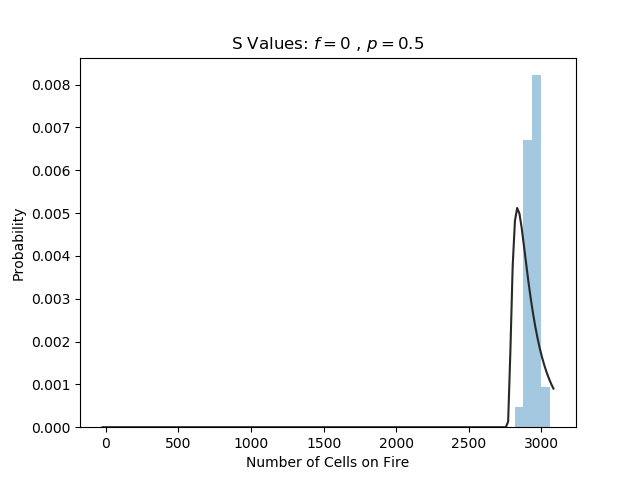
\includegraphics[scale=0.7]{/home/mitchell/Documents/masters/statmech/first/Case_1_NoKDE.png}
\caption{PDF of $100 \times 100$ simulation}
\end{figure}

\subsubsection{Case 2:}

\begin{figure}[H]
\centering
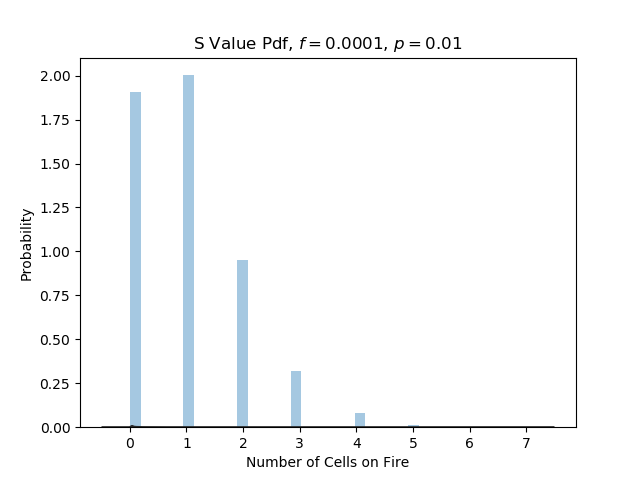
\includegraphics[scale=0.7]{/home/mitchell/Documents/masters/statmech/first/Case_2_NoKDE.png}\caption{PDF of $100 \times 100$ simulation}
\end{figure}

\subsubsection{Case 3:}

\begin{figure}[H]
\centering
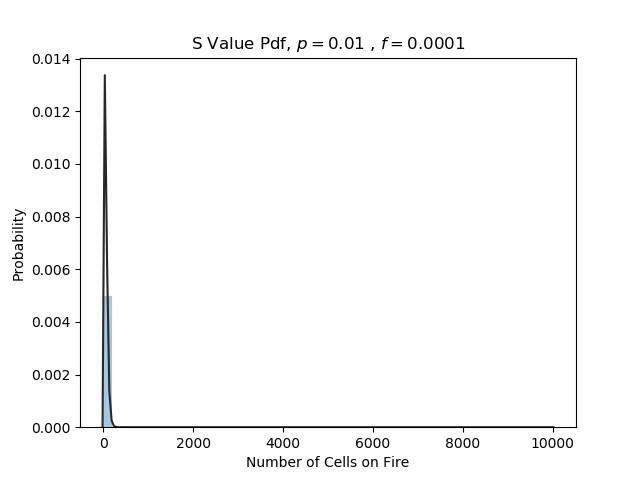
\includegraphics[scale=0.7]{/home/mitchell/Documents/masters/statmech/first/Case_3_NoKDE.png}
\caption{PDF of $100 \times 100$ simulation}
\end{figure}


%%%%%%%%%%%%%%%%%%%%%%%%%%%%%%%%%%%%%%%%%%%%%%%%%%%%%%%%%%%%%%%%%%%%%%
\section{Question 6}
\label{sec:question6}
%%%%%%%%%%%%%%%%%%%%%%%%%%%%%%%%%%%%%%%%%%%%%%%%%%%%%%%%%%%%%%%%%%%%%%


%%%%%%%%%%%%%%%%%%%%%%%%%%%
\subsection{Question 6}
\label{sec:question6:subsec:parta}
%%%%%%%%%%%%%%%%%%%%%%%%%%%

\subsubsection{Case 1:}
For case 1, the inital fire spreads slower than the growth of the forest, and so the initial fire will never die out. When you watch the fire simulation, it appears that you have a continuous fire across the whole sim. This makes sense, since the forest is regenerating at a very rapid rate, and so the fire won't ever exhaust its supply. Its equilibrium state consists of being perpetually on fire, and based on the number of cells on fire, it appears that approximately 1/3 of the simulation is burning once this equilibrium state is reached.

\subsubsection{Case 2:}
For case 2, the probabilities used were taken so that the ratio of $p/f$ was at least 100. This ensured they were sufficiently large enough and satistfied the condition $0 << p << f << 1$. Qualitatively, the fire initially burns through the forest, before settling into an equilibrium. Because the growth is so slow, it is unlikely that the forest will grow with clumps, and so when a fire starts, it will likely ignite only a single cell before burning itself out. 

\subsubsection{Case 3:}
For case 3, the probabilites were reverse from the previous case. Qualitatively, this meant that the forest was growing faster than the fires might start. Once the initial forest burnt away, it regrows faster than in case 2. However, it still takes a while to get to a critical point where it cascades readily, and when it does, virtually the entire forest burns away again. This means that for the large majority of cases, there will be no fire. 

%%%%%%%%%%%%%%%%%%%%%%%%%%%%%%%%%%%%%%%%%%%%%%%%%%%%%%%%%%%%%%%%%%%%%%
\section{Question 7}
\label{sec:question7}
%%%%%%%%%%%%%%%%%%%%%%%%%%%%%%%%%%%%%%%%%%%%%%%%%%%%%%%%%%%%%%%%%%%%%%


%%%%%%%%%%%%%%%%%%%%%%%%%%%
\subsection{Question 7}
\label{sec:question7:subsec:parta}
%%%%%%%%%%%%%%%%%%%%%%%%%%%

The Waiting Times can be visualised by treating the system ergodically, and measuring the waiting times for each cell of a given system after it has run for a sufficiently long time and therefore reached equilibrium. Again I made efforts to normalise the graph, but it wasn't successful in one case. 
\subsubsection{Case 1: }

\begin{figure}[H]
\centering
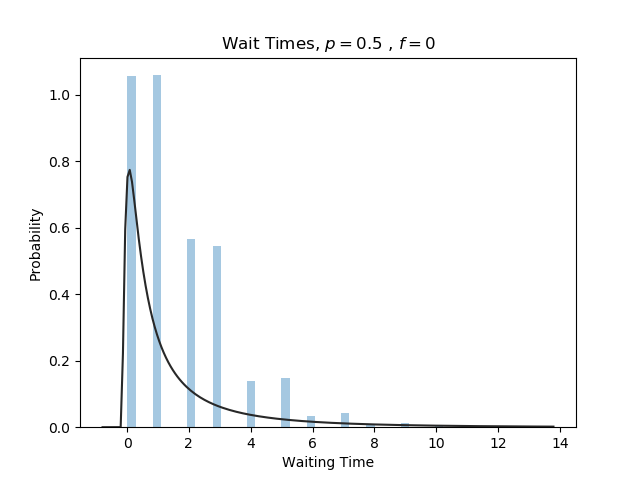
\includegraphics[scale=0.7]{/home/mitchell/Documents/masters/statmech/first/Case_1_Wait_NoKDE.png}
\caption{PDF of $100 \times 100$ simulation wait times}
\end{figure}
\subsubsection{Case 2: }

\begin{figure}[H]
\centering
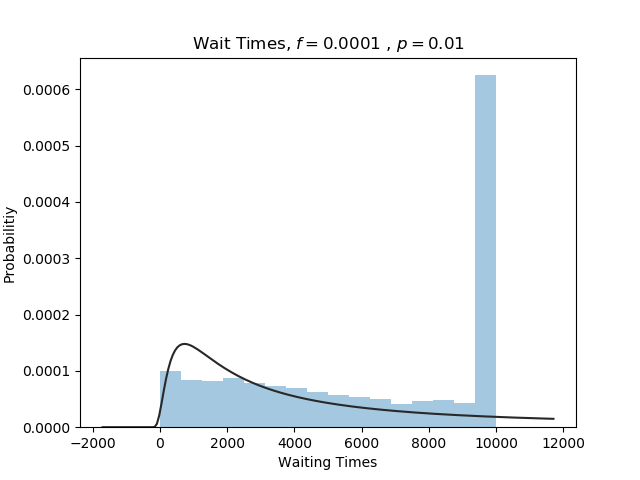
\includegraphics[scale=0.7]{/home/mitchell/Documents/masters/statmech/first/Case_2_Wait_NoKDE.png}
\caption{PDF of $100 \times 100$ simulation wait times}
\end{figure}
\subsubsection{Case 3: }

\begin{figure}[H]
\centering
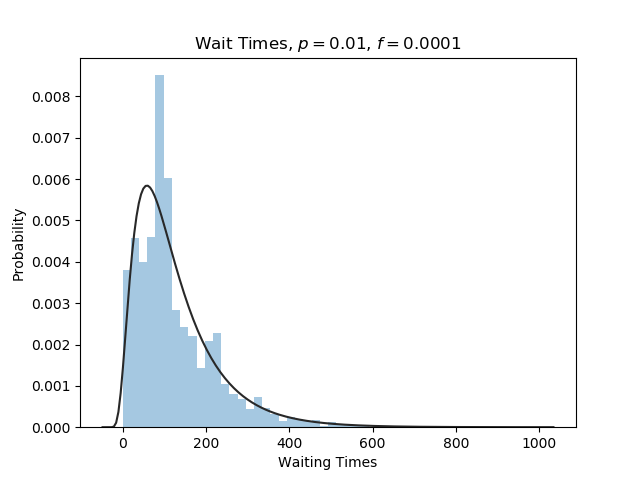
\includegraphics[scale=0.7]{/home/mitchell/Documents/masters/statmech/first/Case_3_Wait_NoKDE.png}
\caption{PDF of $100 \times 100$ simulation wait times}
\end{figure}

In all three cases, the simulation was run for 10000 before it was measured. What we see is that for the case where it is very likely that a cell will be on fire, the wait times are very low, with a peak at 0. For a system which regenerates slowly, this will be spread out much more, indeed, some cells might never catch fire again, which is what we see in the PDF of the wait times for Case 2. For Case 3, the cascades occur much more frequently, and so the waiting times are much less spread towards the higher times. 

 %%%%%%%%%%%%%%%%%%%%%%%%%%%%%%%%%%%%%%%%%%%%%%%%%%%%%%%%%%%%%%%%%%%%%%
\section{Question 8}
\label{sec:question8}
%%%%%%%%%%%%%%%%%%%%%%%%%%%%%%%%%%%%%%%%%%%%%%%%%%%%%%%%%%%%%%%%%%%%%%


%%%%%%%%%%%%%%%%%%%%%%%%%%%
\subsection{Question 8}
\label{sec:question8:subsec:parta}
%%%%%%%%%%%%%%%%%%%%%%%%%%%

On average, the behaviour of the green and red sites will be governed by differential equations which broadly speaking follow an \textit{inflow} - \textit{outflow} model. 

For Green Sites, the inflow is proportional to $1-x_g -x_r$, since this number is representative of the number of cells that are black, related by the probability of them being converted from black to green $p$. Therefore the inflow is $p(1-x_g-x_r)$. 

Outflow is given by the sum of the probability of green cells turning red $f x_g$ and the probability of finding a green and red site next to each other $4 x_g x_r$. This therefore gives the differential equation governing the green sites as 
\begin{equation}\label{eq:xg}
\frac{d x_g}{dt } = p (1 - x_g - x_r) - f x_g - 4 x_g x_r 
\end{equation}

For Red Sites, the inflow is the same as the outflow from green, in this case $f x_g + 4 x_g x_r $ and the outflow is given by $x_r$ since all red sites convert to black immediately.

This therefore makes the differential equation 
\begin{equation}\label{eq:xr}
\frac{d x_r}{d t} = f x_g + 4 x_r x_g - x_r
\end{equation}

Which are both exactly what we are expecting
%%%%%%%%%%%%%%%%%%%%%%%%%%%%%%%%%%%%%%%%%%%%%%%%%%%%%%%%%%%%%%%%%%%%%%
\section{Question 9}
\label{sec:question9}
%%%%%%%%%%%%%%%%%%%%%%%%%%%%%%%%%%%%%%%%%%%%%%%%%%%%%%%%%%%%%%%%%%%%%%


%%%%%%%%%%%%%%%%%%%%%%%%%%%
\subsection{Question 9}
\label{sec:question9:subsec:parta}
%%%%%%%%%%%%%%%%%%%%%%%%%%%
The steady state solutions can be found by setting the left hand sides of \eqref{eq:xg} and \eqref{eq:xr} to zero, and solving the resulting system of equations.

\begin{align}
0 &= - f x_g - 4 x_g x_r + p( 1-x_g - x_r) \label{eq:sys_1} \\
0 &= -x_r + f x_g + 4 x_g x_r  \label{eq:sys_2} \\
\end{align} 
Taking \eqref{eq:sys_2} we see
$$ 4 x_g x_r = x_r - f x_g $$
which we can substitute into \eqref{eq:sys_1}, which yields
\begin{align*}
x_r (1 + p) &= p - p x_g \\
x_r &= \frac{p(1-x_g)}{p+1}
\end{align*}
Substituting this now into \eqref{eq:sys_2} and expanding gives us a quadratic for $x_g$ as follows
\begin{align*}
0 &= - \frac{p(1-x_g)}{p+1} + f x_g + 4 x_g \frac{p(1-x_g)}{p+1} \\ 
&=  - p + p x_g + p f x_g + f x_g + 4 p x_g - 4 p x_g^2 \\
\Rightarrow x_g &= \frac{- (4 p + p + f + f p) \pm \sqrt{(4 p + p + f + f p)^2 - 4 (-4p) p }}{-8p} \\
\Rightarrow x_r &= \frac{p}{p+1} \left(1 + \frac{- (4 p + p + f + f p) \pm \sqrt{(4 p + p + f + f p)^2 - 4 (-4p) p }}{-8p} \right)
\end{align*}

\par For the case where $f= 0 $ and $p = 0.5$, we obtain two steady state solutions 
\begin{align}
x_g &= \frac{1}{4} & x_r = \frac{1}{4}  \\
x_g &= 1 & x_r = 0 \label{eq:case_1:ss}
\end{align}

This makes some sense, since if we have a case where we don't initialise a cell on fire in the system, it will just grow until the entire automaton is green cells, with no fire cells. 
However, if you initialise the automaton with a single cell on fire, it will exist in roughly a state where one quater of the cells are on fire and one quater of the cells are green. 
\par This contrasts slightly with the numbers we observe, where the number of cells on fire are approximately one third.

\par For the case where $f = 0.01$ and $p = 0.0001$, we again obtain two steady state solutions 
\begin{align}
x_g &\approx 0.0095     &x_r\approx 0.000099 \label{eq:case_2} \\
x_g &\approx 26.243    &x_r\approx -0.0025  
\end{align}
We can immediately discount the last solution, since you cannot have a fraction of cells over 100\% or under 0. If we consider what this looks like with respect to our PDF, this means that about $0.01\%$ of the cells will be red. 
\par When we compare this to our PDF directly, this is close, but not exactly correct. The PDF has approximately $0.01\%$ of cells (by counting directly, this is of the order 1-10), so there are actually slightly more.

\par For the case where $f = 0.0001$ and $p = 0.01$, we again obtain two steady state solutions 
\begin{align}
x_g &\approx 0.249 & x_r \approx 0.000743\\
x_g &\approx 1.003 & x_r \approx -0.000036
\end{align}
Again, we immediately discard the second solution. In this case, we expect approximately $0.07 \% $ of the system to be on fire in the long run. 

\par Comparing this to our PDF, it appears that there is a bin which sits at roughly this number which is the most populous. Given the scale, it is somewhat difficult to see, but we expect that $0.07\%$ of the simulation to correspond to roughly of the order 10 red cells, which is seems like it does. 


\par For all three cases, the actual number of red cells is slightly higher than the predicted value, likely due to the inherent instability of the system. But to first order, the approximations made are sufficient to qualitatively describe the system.
%%%%%%%%%%%%%%%%%%%%%%%%%%%%%%%%%%%%%%%%%%%%%%%%%%%%%%%%%%%%%%%%%%%%%%
\section{Question 10}
\label{sec:question10}
%%%%%%%%%%%%%%%%%%%%%%%%%%%%%%%%%%%%%%%%%%%%%%%%%%%%%%%%%%%%%%%%%%%%%%

%%%%%%%%%%%%%%%%%%%%%%%%%%%
\subsection{Question 19}
\label{sec:question10:subsec:parta}
%%%%%%%%%%%%%%%%%%%%%%%%%%%
In order to make the system more realistic, I would introduce a couple of changes to the simulation:
\begin{enumerate}
\item Allow for fire to jump, if for example, it was drive by wind, or some other factor. This would account for the fact that there are additional driving factors in the system other than just the probability of random fire generation. 
\item Allow for increased clumping in regrowth, by esssentially preferencing the probability of trees growing next to an existing cell with trees. This would probably be incorporated by lowering the regeneration probability for a cell next to a green cell. Using the convolution method would actually be better for this, since it would allow for varying probability depending the number of neighboring green cells. 
\item Make the tree growth time and the fire extinguishing time different orders of magnitude, since a tree cannot grow in the time it takes for a fire to burn through it. This correction perhaps needs to account for the number of neighboring fires, or neighboring forested cells. This fine tuning would require a bit more research into the precise conditions that might exist in the real world, to get a sense of the fire ignition probability and forest regeneration probability.
\end{enumerate}

\end{document}
